% vim: ts=2:sw=2:tw=80:et
\thispagestyle{fancy}
\pagestyle{fancy}


\section{Executing}\label{sec:quick:exec}
Executing Arbwave involves simply executing the \verb|run.py| script found in
the main directory of the Arbwave package.  On most installations, this can
simply be started as an executable script, but may also be started as something
like \verb|python ./run.py|.  Various commandline parameters may also be
specified in order to query the version, specify the log level, or modify the
functionality of Arbwave in various ways.  Sec.~\ref{sec:overview:cmdline} of
Chap.~\ref{chap:op-overview} discusses the various commandline options in
more depth.


\section{Simulated Mode}
One of the commandline options discussed in Chap.~\ref{chap:op-overview}
(\verb|--simulated|)
causes Arbwave to execute in \textbf{Simulated Mode}.  \textbf{Simulated Mode}
operation allows a user to experiment with various waveforms without requiring
or affecting any actual hardware.

\begin{figure}[htb!]
  \centerline{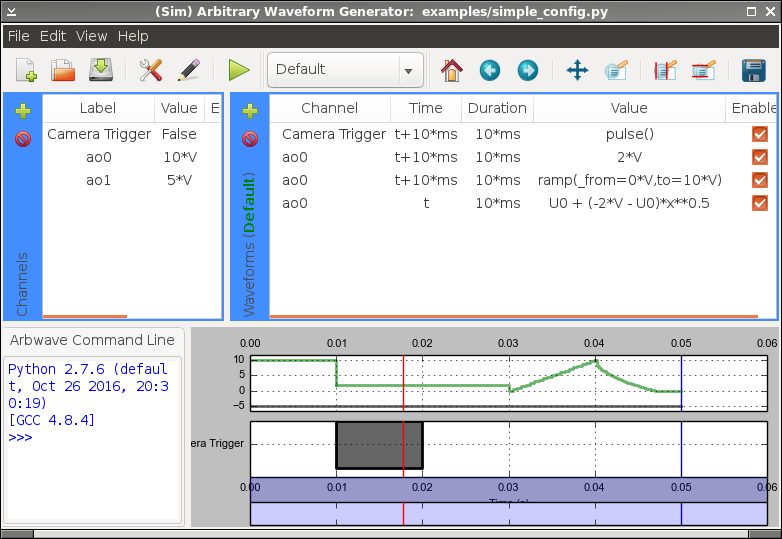
\includegraphics[width=.8\textwidth]{figures/main-simple-config}}
  \caption{Main window when initially loading ``simple-config.py'' in simulated
  mode.}
  \label{fig:quick:main-simple-config}
\end{figure}


In order to get at least a quick feel of what Arbwave is like, it can be very
helpful to run in \textbf{Simulated Mode} with one of the packaged examples.  The
simulated waveforms can be modified to explore Arbwave capabilities.

To do this, use the \verb|--simulated| command line.  There are two ways for you
to load up one of the examples.
\begin{enumerate}
  \item Add the filename of one of the examples on the command line, such as:\\
    \begin{verbatim}
    run.py --simulated examples/simple_config.py
    \end{verbatim}
    or perhaps:
    \begin{verbatim}
    run.py --simulated examples/simple_ni_only_config.py
    \end{verbatim}
    After loading the one of these examples, you should see the main window,
    such as shown in Fig.~\ref{fig:quick:main-simple-config} for \verb|simple_config.py|.
  \item Start Arbwave up in simulated mode with \verb|run.py --simulated| and
  then use the Open menu option.  Browse to \verb|examples/| and select one of
  the included examples.  As of this writing there are two examples, \verb|simple_config.py|
  and \verb|simple_ni_only_config.py|.  The former includes channels for a camera trigger device
  and two analog outputs.  The latter has channels for an analog output and a digital output.
\end{enumerate}
